\section{Instance Class Reference}
\label{classInstance}\index{Instance@{Instance}}
Inheritance diagram for Instance:\begin{figure}[H]
\begin{center}
\leavevmode
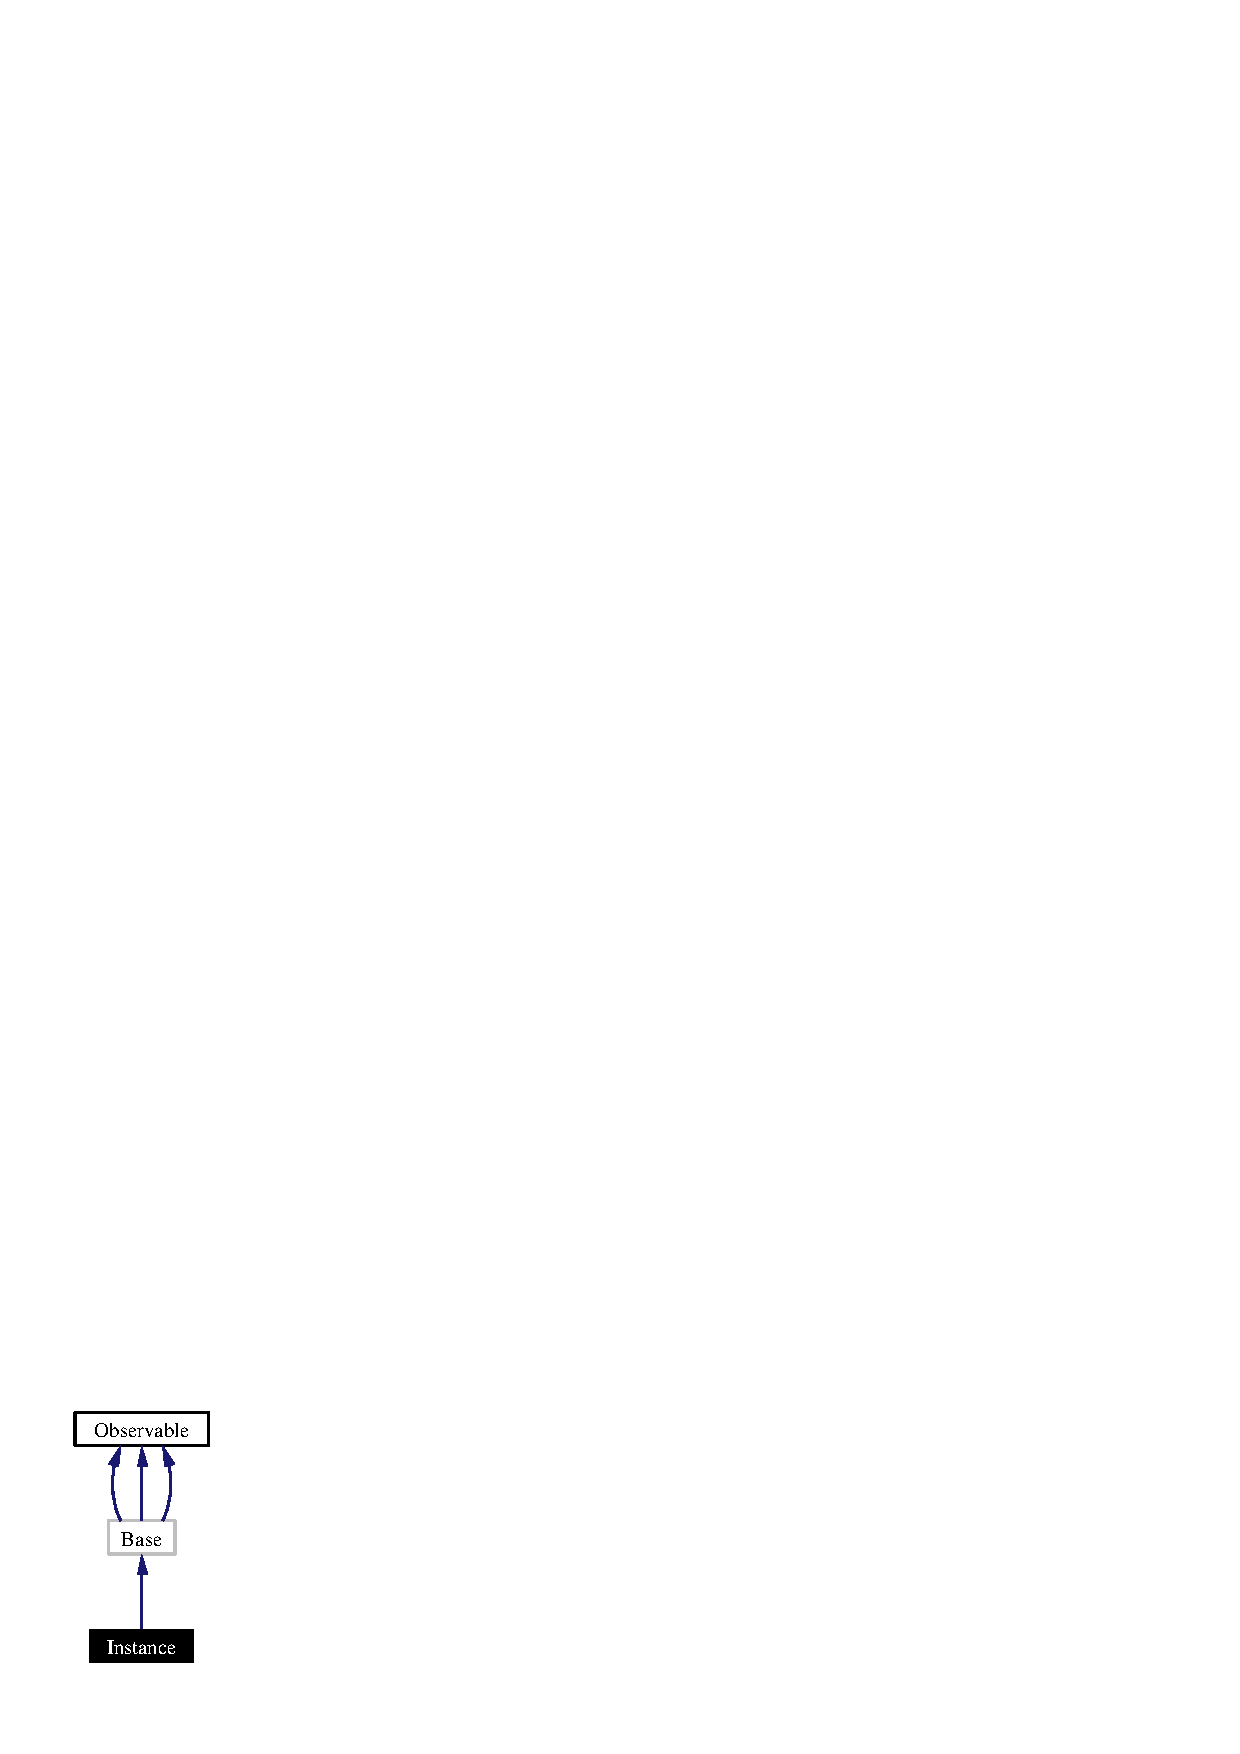
\includegraphics[width=50pt]{classInstance__inherit__graph}
\end{center}
\end{figure}
Collaboration diagram for Instance:\begin{figure}[H]
\begin{center}
\leavevmode
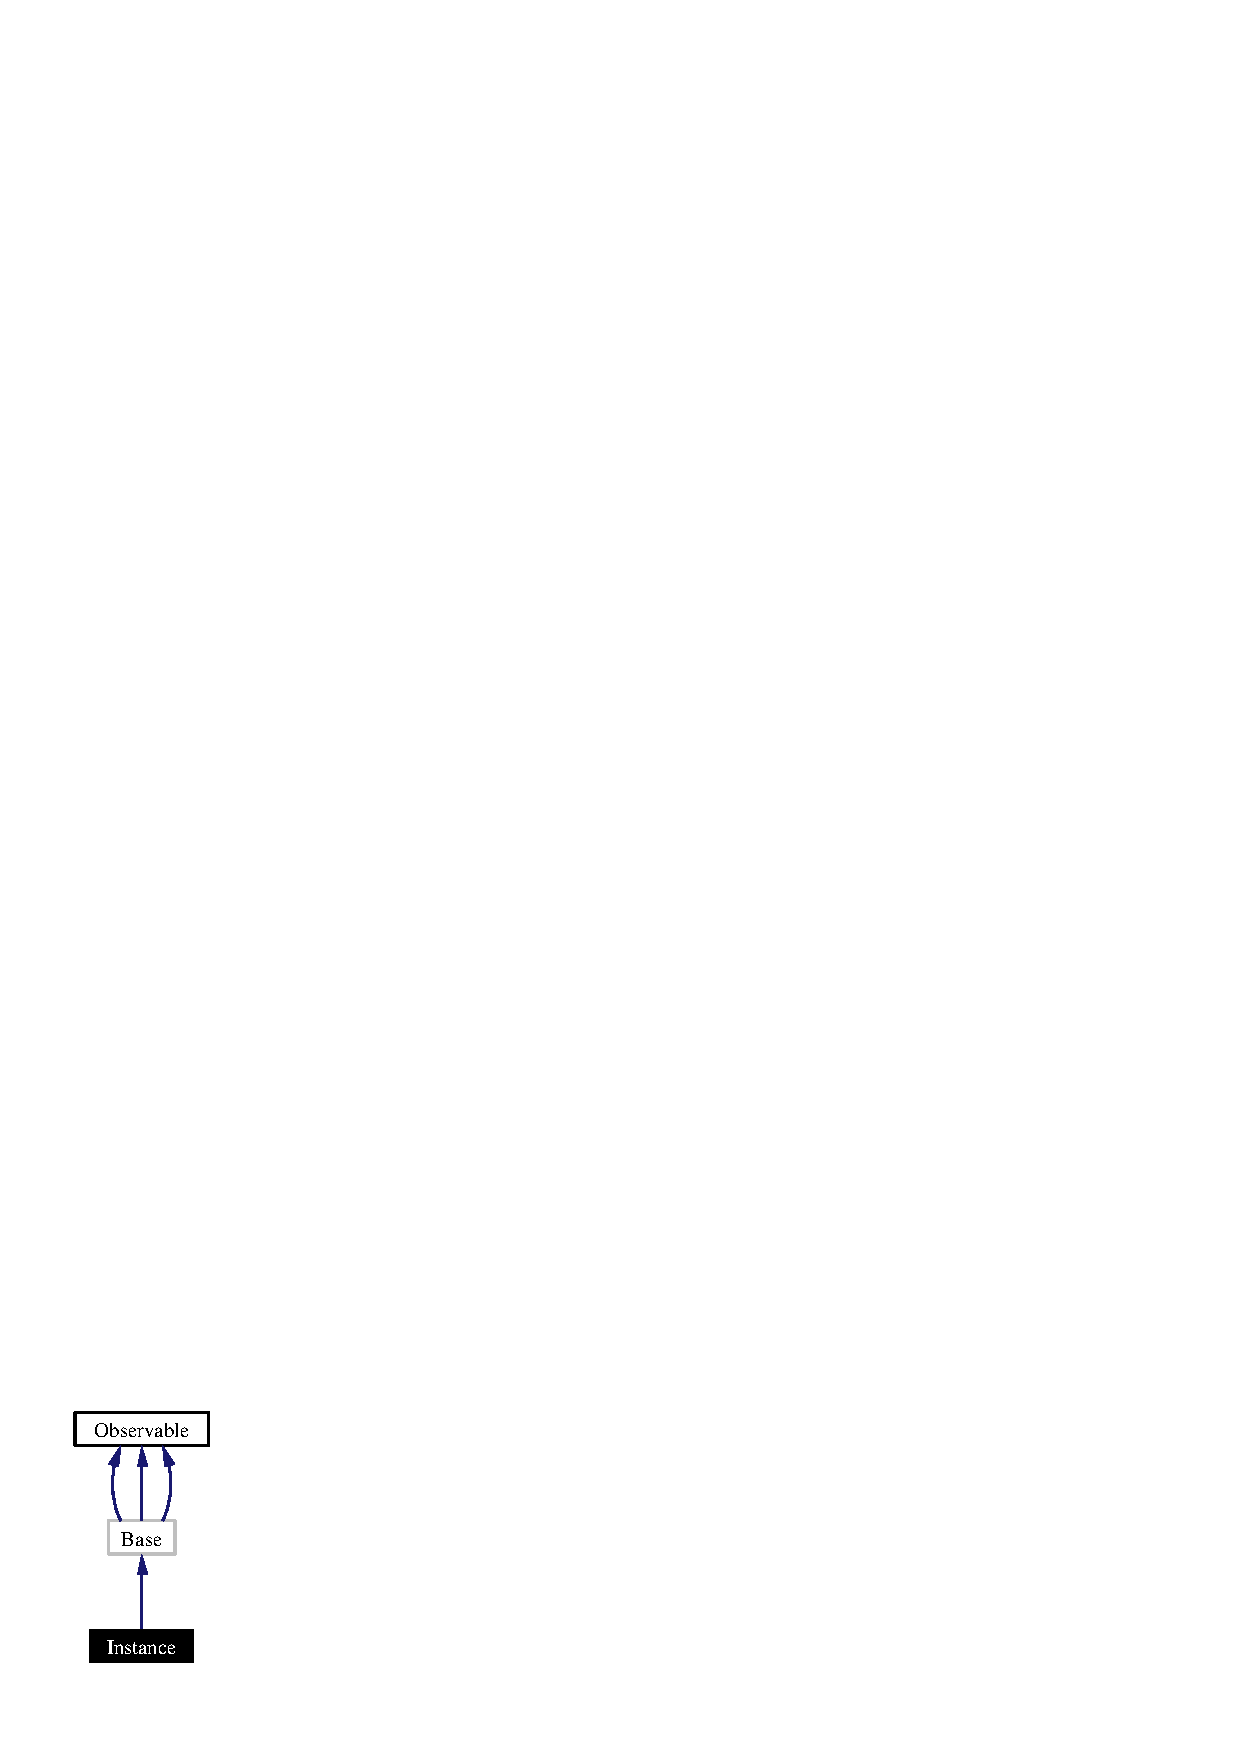
\includegraphics[width=50pt]{classInstance__coll__graph}
\end{center}
\end{figure}
\subsection*{Public Member Functions}
\begin{CompactItemize}
\item 
\index{Instance@{Instance}!Instance@{Instance}}\index{Instance@{Instance}!Instance@{Instance}}
{\bf Instance} (\$db)\label{classInstance_a0}

\item 
{\bf get\-Instance} (\$instance\-Id)
\item 
{\bf set\-Next\-Activity} (\$actname)
\item 
{\bf set\-Next\-User} (\$user)
\item 
{\bf set} (\$name,\$value)
\item 
{\bf get} (\$name)
\item 
{\bf get\-Activities} ()
\item 
{\bf get\-Status} ()
\item 
{\bf set\-Status} (\$status)
\item 
{\bf get\-Instance\-Id} ()
\item 
{\bf get\-Process\-Id} ()
\item 
{\bf get\-Owner} ()
\item 
{\bf set\-Owner} (\$user)
\item 
{\bf set\-Activity\-User} (\$activity\-Id,\$theuser)
\item 
{\bf get\-Activity\-User} (\$activity\-Id)
\item 
{\bf set\-Activity\-Status} (\$activity\-Id,\$status)
\item 
{\bf get\-Activity\-Status} (\$activity\-Id)
\item 
{\bf set\-Activity\-Started} (\$activity\-Id)
\item 
{\bf get\-Activity\-Started} (\$activity\-Id)
\item 
{\bf set\-Started} (\$time)
\item 
{\bf get\-Started} ()
\item 
{\bf set\-Ended} (\$time)
\item 
{\bf get\-Ended} ()
\item 
{\bf complete} (\$activity\-Id=0,\$force=false,\$addworkitem=true)
\item 
{\bf terminate} ()
\item 
{\bf send\-To} (\$from,\$activity\-Id,\$split=false)
\item 
{\bf get\_\-instance\_\-comment} (\$c\-Id)
\item 
{\bf replace\_\-instance\_\-comment} (\$c\-Id,\$activity\-Id,\$activity,\$user,\$title,\$comment)
\item 
{\bf remove\_\-instance\_\-comment} (\$c\-Id)
\item 
{\bf get\_\-instance\_\-comments} ()
\end{CompactItemize}
\subsection*{Public Attributes}
\begin{CompactItemize}
\item 
\index{properties@{properties}!Instance@{Instance}}\index{Instance@{Instance}!properties@{properties}}
{\bf properties} = Array()\label{classInstance_m0}

\item 
\index{owner@{owner}!Instance@{Instance}}\index{Instance@{Instance}!owner@{owner}}
{\bf owner} = ''\label{classInstance_m1}

\item 
\index{status@{status}!Instance@{Instance}}\index{Instance@{Instance}!status@{status}}
{\bf status} = ''\label{classInstance_m2}

\item 
\index{started@{started}!Instance@{Instance}}\index{Instance@{Instance}!started@{started}}
{\bf started}\label{classInstance_m3}

\item 
\index{nextActivity@{nextActivity}!Instance@{Instance}}\index{Instance@{Instance}!nextActivity@{nextActivity}}
{\bf next\-Activity}\label{classInstance_m4}

\item 
\index{nextUser@{nextUser}!Instance@{Instance}}\index{Instance@{Instance}!nextUser@{nextUser}}
{\bf next\-User}\label{classInstance_m5}

\item 
\index{ended@{ended}!Instance@{Instance}}\index{Instance@{Instance}!ended@{ended}}
{\bf ended}\label{classInstance_m6}

\item 
\index{activities@{activities}!Instance@{Instance}}\index{Instance@{Instance}!activities@{activities}}
{\bf activities} = Array()\label{classInstance_m7}

\begin{CompactList}\small\item\em Array of asocs(activity\-Id,status,started,user).\item\end{CompactList}\item 
\index{pId@{pId}!Instance@{Instance}}\index{Instance@{Instance}!pId@{pId}}
{\bf p\-Id}\label{classInstance_m8}

\item 
\index{instanceId@{instanceId}!Instance@{Instance}}\index{Instance@{Instance}!instanceId@{instanceId}}
{\bf instance\-Id} = 0\label{classInstance_m9}

\item 
\index{workitems@{workitems}!Instance@{Instance}}\index{Instance@{Instance}!workitems@{workitems}}
{\bf workitems} = Array()\label{classInstance_m10}

\begin{CompactList}\small\item\em An array of workitem ids.\item\end{CompactList}\end{CompactItemize}


\subsection{Detailed Description}
This class represents a process instance, it is used when any activity is executed. The \$instance object is created representing the instance of a process being executed in the activity or even a to-be-created instance if the activity is a start activity. 



Definition at line 10 of file Instance.php.

\subsection{Member Function Documentation}
\index{Instance@{Instance}!complete@{complete}}
\index{complete@{complete}!Instance@{Instance}}
\subsubsection{\setlength{\rightskip}{0pt plus 5cm}Instance::complete (\$ {\em activity\-Id} = 0, \$ {\em force} = false, \$ {\em addworkitem} = true)}\label{classInstance_a23}


Completes an activity, normally from any activity you should call this function without arguments. The arguments are explained just in case. \$activity\-Id is the activity that is being completed, when this is not passed the engine takes it from the \$\_\-REQUEST array,all activities are executed passing the activity\-Id in the URI. \$force indicates that the instance must be routed no matter if the activity is auto-routing or not. This is used when \char`\"{}sending\char`\"{} an instance from a non-auto-routed activity to the next activity. \$addworkitem indicates if a workitem should be added for the completed activity. YOU MUST NOT CALL {\bf complete()} for non-interactive activities since the engine does automatically complete automatic activities after executing them. 

Definition at line 384 of file Instance.php.

References get\-Owner(), get\-Started(), send\-To(), set\-Activity\-Status(), and terminate().

Referenced by send\-To().\index{Instance@{Instance}!get@{get}}
\index{get@{get}!Instance@{Instance}}
\subsubsection{\setlength{\rightskip}{0pt plus 5cm}Instance::get (\$ {\em name})}\label{classInstance_a5}


Gets the value of an instance property. 

Definition at line 150 of file Instance.php.\index{Instance@{Instance}!get_instance_comment@{get\_\-instance\_\-comment}}
\index{get_instance_comment@{get\_\-instance\_\-comment}!Instance@{Instance}}
\subsubsection{\setlength{\rightskip}{0pt plus 5cm}Instance::get\_\-instance\_\-comment (\$ {\em c\-Id})}\label{classInstance_a26}


Gets a comment for this instance 

Definition at line 610 of file Instance.php.\index{Instance@{Instance}!get_instance_comments@{get\_\-instance\_\-comments}}
\index{get_instance_comments@{get\_\-instance\_\-comments}!Instance@{Instance}}
\subsubsection{\setlength{\rightskip}{0pt plus 5cm}Instance::get\_\-instance\_\-comments ()}\label{classInstance_a29}


Lists instance comments 

Definition at line 662 of file Instance.php.\index{Instance@{Instance}!getActivities@{getActivities}}
\index{getActivities@{getActivities}!Instance@{Instance}}
\subsubsection{\setlength{\rightskip}{0pt plus 5cm}Instance::get\-Activities ()}\label{classInstance_a6}


Returns an array of asocs describing the activities where the instance is present, can be more than one activity if the instance was \char`\"{}splitted\char`\"{} 

Definition at line 163 of file Instance.php.\index{Instance@{Instance}!getActivityStarted@{getActivityStarted}}
\index{getActivityStarted@{getActivityStarted}!Instance@{Instance}}
\subsubsection{\setlength{\rightskip}{0pt plus 5cm}Instance::get\-Activity\-Started (\$ {\em activity\-Id})}\label{classInstance_a18}


Gets the Unix timstamp of the starting time for the given activity. 

Definition at line 306 of file Instance.php.\index{Instance@{Instance}!getActivityStatus@{getActivityStatus}}
\index{getActivityStatus@{getActivityStatus}!Instance@{Instance}}
\subsubsection{\setlength{\rightskip}{0pt plus 5cm}Instance::get\-Activity\-Status (\$ {\em activity\-Id})}\label{classInstance_a16}


Gets the status of the instance in some activity, can be 'running' or 'completed' 

Definition at line 278 of file Instance.php.\index{Instance@{Instance}!getActivityUser@{getActivityUser}}
\index{getActivityUser@{getActivityUser}!Instance@{Instance}}
\subsubsection{\setlength{\rightskip}{0pt plus 5cm}Instance::get\-Activity\-User (\$ {\em activity\-Id})}\label{classInstance_a14}


Returns the user that must execute or is already executing an activity wherethis instance is present. 

Definition at line 248 of file Instance.php.\index{Instance@{Instance}!getEnded@{getEnded}}
\index{getEnded@{getEnded}!Instance@{Instance}}
\subsubsection{\setlength{\rightskip}{0pt plus 5cm}Instance::get\-Ended ()}\label{classInstance_a22}


Gets the end time of the instance (when the process was completed) 

Definition at line 361 of file Instance.php.\index{Instance@{Instance}!getInstance@{getInstance}}
\index{getInstance@{getInstance}!Instance@{Instance}}
\subsubsection{\setlength{\rightskip}{0pt plus 5cm}Instance::get\-Instance (\$ {\em instance\-Id})}\label{classInstance_a1}


Method used to load an instance data from the database. 

Definition at line 33 of file Instance.php.

Referenced by send\-To().\index{Instance@{Instance}!getInstanceId@{getInstanceId}}
\index{getInstanceId@{getInstanceId}!Instance@{Instance}}
\subsubsection{\setlength{\rightskip}{0pt plus 5cm}Instance::get\-Instance\-Id ()}\label{classInstance_a9}


Returns the instance\-Id 

Definition at line 193 of file Instance.php.\index{Instance@{Instance}!getOwner@{getOwner}}
\index{getOwner@{getOwner}!Instance@{Instance}}
\subsubsection{\setlength{\rightskip}{0pt plus 5cm}Instance::get\-Owner ()}\label{classInstance_a11}


Returns the user that created the instance 

Definition at line 209 of file Instance.php.

Referenced by complete().\index{Instance@{Instance}!getProcessId@{getProcessId}}
\index{getProcessId@{getProcessId}!Instance@{Instance}}
\subsubsection{\setlength{\rightskip}{0pt plus 5cm}Instance::get\-Process\-Id ()}\label{classInstance_a10}


Returns the process\-Id for this instance 

Definition at line 201 of file Instance.php.\index{Instance@{Instance}!getStarted@{getStarted}}
\index{getStarted@{getStarted}!Instance@{Instance}}
\subsubsection{\setlength{\rightskip}{0pt plus 5cm}Instance::get\-Started ()}\label{classInstance_a20}


Gets the time where the instance was started (Unix timestamp) 

Definition at line 343 of file Instance.php.

Referenced by complete().\index{Instance@{Instance}!getStatus@{getStatus}}
\index{getStatus@{getStatus}!Instance@{Instance}}
\subsubsection{\setlength{\rightskip}{0pt plus 5cm}Instance::get\-Status ()}\label{classInstance_a7}


Gets the instance status can be 'completed', 'active', 'aborted' or 'exception' 

Definition at line 172 of file Instance.php.\index{Instance@{Instance}!remove_instance_comment@{remove\_\-instance\_\-comment}}
\index{remove_instance_comment@{remove\_\-instance\_\-comment}!Instance@{Instance}}
\subsubsection{\setlength{\rightskip}{0pt plus 5cm}Instance::remove\_\-instance\_\-comment (\$ {\em c\-Id})}\label{classInstance_a28}


Removes an instance comment 

Definition at line 652 of file Instance.php.\index{Instance@{Instance}!replace_instance_comment@{replace\_\-instance\_\-comment}}
\index{replace_instance_comment@{replace\_\-instance\_\-comment}!Instance@{Instance}}
\subsubsection{\setlength{\rightskip}{0pt plus 5cm}Instance::replace\_\-instance\_\-comment (\$ {\em c\-Id}, \$ {\em activity\-Id}, \$ {\em activity}, \$ {\em user}, \$ {\em title}, \$ {\em comment})}\label{classInstance_a27}


Inserts or updates an instance comment 

Definition at line 623 of file Instance.php.\index{Instance@{Instance}!sendTo@{sendTo}}
\index{sendTo@{sendTo}!Instance@{Instance}}
\subsubsection{\setlength{\rightskip}{0pt plus 5cm}Instance::send\-To (\$ {\em from}, \$ {\em activity\-Id}, \$ {\em split} = false)}\label{classInstance_a25}


Sends the instance from some activity to another activity. You should not call this method unless you know very very well what you are doing. 

Definition at line 504 of file Instance.php.

References complete(), and get\-Instance().

Referenced by complete().\index{Instance@{Instance}!set@{set}}
\index{set@{set}!Instance@{Instance}}
\subsubsection{\setlength{\rightskip}{0pt plus 5cm}Instance::set (\$ {\em name}, \$ {\em value})}\label{classInstance_a4}


Sets a property in this instance. This method is used in activities to set instance properties. Instance properties are inemdiately serialized. 

Definition at line 139 of file Instance.php.\index{Instance@{Instance}!setActivityStarted@{setActivityStarted}}
\index{setActivityStarted@{setActivityStarted}!Instance@{Instance}}
\subsubsection{\setlength{\rightskip}{0pt plus 5cm}Instance::set\-Activity\-Started (\$ {\em activity\-Id})}\label{classInstance_a17}


Resets the start time of the activity indicated to the current time. 

Definition at line 291 of file Instance.php.\index{Instance@{Instance}!setActivityStatus@{setActivityStatus}}
\index{setActivityStatus@{setActivityStatus}!Instance@{Instance}}
\subsubsection{\setlength{\rightskip}{0pt plus 5cm}Instance::set\-Activity\-Status (\$ {\em activity\-Id}, \$ {\em status})}\label{classInstance_a15}


Sets the status of the instance in some activity, can be 'running' or 'completed' 

Definition at line 262 of file Instance.php.

Referenced by complete().\index{Instance@{Instance}!setActivityUser@{setActivityUser}}
\index{setActivityUser@{setActivityUser}!Instance@{Instance}}
\subsubsection{\setlength{\rightskip}{0pt plus 5cm}Instance::set\-Activity\-User (\$ {\em activity\-Id}, \$ {\em theuser})}\label{classInstance_a13}


Sets the user that must execute the activity indicated by the activity\-Id. Note that the instance MUST be present in the activity to set the user, you can't program who will execute an activity. 

Definition at line 231 of file Instance.php.\index{Instance@{Instance}!setEnded@{setEnded}}
\index{setEnded@{setEnded}!Instance@{Instance}}
\subsubsection{\setlength{\rightskip}{0pt plus 5cm}Instance::set\-Ended (\$ {\em time})}\label{classInstance_a21}


Sets the end time of the instance (when the process was completed) 

Definition at line 351 of file Instance.php.\index{Instance@{Instance}!setNextActivity@{setNextActivity}}
\index{setNextActivity@{setNextActivity}!Instance@{Instance}}
\subsubsection{\setlength{\rightskip}{0pt plus 5cm}Instance::set\-Next\-Activity (\$ {\em actname})}\label{classInstance_a2}


Sets the next activity to be executed, if the current activity is a switch activity the {\bf complete()} method will use the activity setted in this method as the next activity for the instance. Note that this method receives an activity name as argument. (Not an Id) 

Definition at line 66 of file Instance.php.\index{Instance@{Instance}!setNextUser@{setNextUser}}
\index{setNextUser@{setNextUser}!Instance@{Instance}}
\subsubsection{\setlength{\rightskip}{0pt plus 5cm}Instance::set\-Next\-User (\$ {\em user})}\label{classInstance_a3}


This method can be used to set the user that must perform the next activity of the process. this effectively \char`\"{}assigns\char`\"{} the instance to some user. 

Definition at line 84 of file Instance.php.\index{Instance@{Instance}!setOwner@{setOwner}}
\index{setOwner@{setOwner}!Instance@{Instance}}
\subsubsection{\setlength{\rightskip}{0pt plus 5cm}Instance::set\-Owner (\$ {\em user})}\label{classInstance_a12}


Sets the instance creator user 

Definition at line 217 of file Instance.php.\index{Instance@{Instance}!setStarted@{setStarted}}
\index{setStarted@{setStarted}!Instance@{Instance}}
\subsubsection{\setlength{\rightskip}{0pt plus 5cm}Instance::set\-Started (\$ {\em time})}\label{classInstance_a19}


Sets the time where the instance was started. 

Definition at line 333 of file Instance.php.\index{Instance@{Instance}!setStatus@{setStatus}}
\index{setStatus@{setStatus}!Instance@{Instance}}
\subsubsection{\setlength{\rightskip}{0pt plus 5cm}Instance::set\-Status (\$ {\em status})}\label{classInstance_a8}


Sets the instance status , the value can be: 'completed', 'active', 'aborted' or 'exception' 

Definition at line 181 of file Instance.php.\index{Instance@{Instance}!terminate@{terminate}}
\index{terminate@{terminate}!Instance@{Instance}}
\subsubsection{\setlength{\rightskip}{0pt plus 5cm}Instance::terminate ()}\label{classInstance_a24}


Terminates the instance marking the instance and the process as completed. This is the end of a process. Normally you should not call this method since it is automatically called when an end activity is completed. 

Definition at line 486 of file Instance.php.

Referenced by complete().

The documentation for this class was generated from the following file:\begin{CompactItemize}
\item 
Instance.php\end{CompactItemize}
